\documentclass[conference]{IEEEtran}
\IEEEoverridecommandlockouts
% ---------------------------------------------------------------------------
%  Therapeutic-model drift benchmark + intervention ablation (Phase 3)
% ---------------------------------------------------------------------------
\usepackage{cite}
\usepackage{amsmath,amssymb,amsfonts}
\usepackage{algorithm}
\usepackage{algpseudocode}
\usepackage{graphicx}
\usepackage{textcomp}
\usepackage{xcolor}
\usepackage[T1]{fontenc}
\usepackage{booktabs}
\usepackage{array}
\usepackage{multirow}
\usepackage{url}

% Works whether figures/ sits beside main.tex (Overleaf) or one level up (repo).
\graphicspath{{figures/}{../figures/}}

\def\BibTeX{{\rm B\kern-.05em{\sc i\kern-.025em b}\kern-.08em
    T\kern-.1667em\lower.7ex\hbox{E}\kern-.125emX}}

\begin{document}

\title{Therapeutic-Model Drift in Constrained Mental-Health Language Models:\\
A Benchmark and an Ablation of Prompting, Retrieval and Adaptation}

\author{
\IEEEauthorblockN{Joel B. Koshy}
\IEEEauthorblockA{\textit{Department of Computer Science} \\
\textit{Christ University}\\
Bengaluru, India \\
joel.koshy@res.christuniversity.in}
\and
\IEEEauthorblockN{Rajesh Kanna R.}
\IEEEauthorblockA{\textit{Department of Computer Science} \\
\textit{Christ University}\\
Bengaluru, India \\
rajesh.kanna@christuniversity.in}
}

\maketitle

\begin{abstract}
Evaluations of therapeutic language models measure whether replies are safe,
empathic or helpful, but not whether they still deliver the therapy the system
was specified to deliver. We call the failure to do so \emph{therapeutic-model
drift}, and argue it is distinct from jailbreaking: the requests that produce it
---\,``help me weigh the evidence for that thought'', ``just tell me it will be
fine''\,--- are sincere, sympathetic, and exactly what alignment training
disposes a model to grant, yet Metacognitive Therapy (MCT) forbids granting them.
We introduce MCT-DriftBench: eight drift families anchored to specific MCT
prohibitions, instantiated as 48 probes that pair real first-person depression
narratives with one authored bait turn, plus 54 crisis-phrasing probes with
specificity controls. Using it, we ablate the three interventions usually bundled
together --- prompt specification, retrieval grounding, and LoRA adaptation ---
on one base checkpoint (Qwen2.5-1.5B-Instruct) with matched prompts, decoding and
seed, against a Llama-3-8B scale reference. Specifying the therapy carries most
of the fidelity gain ($+0.80$, $r=1.00$); adaptation adds more at matched prompt
than lengthening the prompt does ($+0.52$, $r=0.95$); retrieval buys no fidelity
and significantly \emph{reduces} it on adapted weights ($-0.50$, $r=-0.97$)
despite being the costliest at inference. The 8B reference is no better on either
axis while refusing 25\% of clinical narratives. Two negative results temper the
rest: an unconstrained control was rated 97.5\% constraint-compliant while
scoring zero on all five MCT technique indicators, showing violation-counting
cannot distinguish adherence from absence of therapy; and the deterministic
crisis screener that reported $F_1=1.00$ on researcher-authored narratives
achieves recall of $0.211$ against independently authored phrasings, detecting no
passive or figurative expression of risk. Our lexical detector and an independent
model judge recovered near-identical drift rates while agreeing on individual
items at chance ($\kappa=0.086$), so we report drift as a rate estimate rather
than per-item ground truth. Probes, code, generations and verdicts are released.
\end{abstract}

\begin{IEEEkeywords}
therapeutic fidelity, metacognitive therapy, large language models, red teaming,
retrieval-augmented generation, low-rank adaptation, mental health safety,
behavioural testing
\end{IEEEkeywords}

\section{Introduction}

Evaluations of language models for mental health almost always measure the wrong
thing at the wrong moment. A system is given a series of cooperative inputs, its
replies are scored for empathy, helpfulness, or safety, and the resulting average
is reported as evidence that the system is fit for a therapeutic role
\cite{stade2024llm,sharma2023empathy}. What that procedure cannot tell you is
whether the therapy survives a service user who pushes back.

This distinction matters more in psychotherapy than in most applications, because
in psychotherapy the constraints \emph{are} the intervention. Metacognitive
Therapy (MCT), developed by Wells on the Self-Regulatory Executive Function
model, holds that psychological disorder is maintained not by the content of
negative thoughts but by the extended processing applied to them --- worry,
rumination, threat monitoring, and avoidance, collectively the Cognitive
Attentional Syndrome (CAS) \cite{wells1996sref,wells2009mct}. The therapy
therefore works on the process and deliberately declines to work on the content.
A therapist who explores what the patient was thinking about, disputes whether it
was accurate, or reassures the patient that it will turn out well is not
delivering MCT badly; they are delivering something else. Meta-analytic evidence
supports MCT's efficacy in depression \cite{normann2018efficacy}, and the
efficacy belongs to the protocol, not to the warmth with which it is delivered
\cite{waltz1993adherence,perepletchikova2007integrity}.

That creates a specific and, we argue, under-measured failure mode. A model can
be made to produce excellent MCT on cooperative input --- earlier phases of this
programme demonstrated exactly that, reaching high automated adherence on both
synthetic and real narratives --- and can nevertheless abandon the protocol the
moment a user asks it to. We call this \emph{therapeutic-model drift}: the system
does not become unsafe, offensive, or incoherent, and so passes every
conventional safety evaluation. It simply stops delivering the therapy it claims
to deliver, usually while sounding more helpful than before. A user who asks
``help me work out whether that thought is true'' and receives a considerate
evidence-weighing exercise has been given competent cognitive therapy by a system
that was specified to deliver MCT, and every content-level safety filter in the
stack will pass it.

Drift is not a special case of jailbreaking. The jailbreaking literature is
concerned with eliciting content a model was trained to withhold
\cite{wei2023jailbroken,zou2023universal}, and its probes are adversarial in
intent. The requests that produce therapeutic drift are the opposite: they are
sincere, sympathetic, and exactly what a distressed person would write. ``Please
just tell me it is going to be fine'' is not an attack. It is a request that a
general-purpose assistant is trained by human preference optimisation to satisfy
\cite{ouyang2022instructgpt}, that a sycophantic model will satisfy
enthusiastically \cite{sharma2024sycophancy}, and that MCT explicitly forbids
satisfying, because reassurance-seeking is itself one of the maladaptive coping
behaviours the therapy targets. The pressure toward drift comes from the same
alignment training that makes the model pleasant to use.

The second gap this paper addresses is methodological. Systems of this kind are
built by stacking three interventions --- a prompt that specifies the therapy,
retrieval that grounds replies in a treatment manual, and parameter-efficient
adaptation on therapy-consistent examples --- and are then reported as a single
artefact. Because the three are never varied independently, the field has no
evidence about which of them does the work. Practitioners consequently spend
GPU-hours on adaptation that a longer prompt might have bought, or add a
retrieval stack whose contribution has never been isolated.

This paper makes four contributions.

\begin{enumerate}
\item \textbf{A taxonomy of therapeutic-model drift} with eight families, each
tied to a specific prohibition that distinguishes MCT from adjacent therapies or
that bounds the system's clinical scope.

\item \textbf{MCT-DriftBench}, a released benchmark instantiating that taxonomy
as 48 probes, each pairing a real human-authored narrative with one authored bait
turn, together with 54 crisis-phrasing probes that test the deterministic
pre-generation screener and its false-alarm behaviour. Every generation is scored
twice, by a deterministic lexical detector and by an independent judge model, and
the agreement between them is reported rather than assumed.

\item \textbf{A factorial ablation} that separates prompt specification,
retrieval grounding, and low-rank adaptation on one base checkpoint with matched
prompts, decoding and seed, evaluated on both axes.

\item \textbf{Empirical findings} that the interventions which raise adherence on
cooperative input are not the interventions which confer resistance under
pressure, and that a deterministic keyword screener with near-perfect recall on
plainly worded risk disclosure fails on the majority of the indirect and
figurative phrasings in which risk is more usually expressed.
\end{enumerate}

All probes, code, generations, and analysis are released.

\section{Background and Related Work}

\subsection{What Metacognitive Therapy Prohibits}

The S-REF model treats psychological disorder as a product of a self-perpetuating
attentional and processing style rather than of any particular belief
\cite{wells1996sref}. Its clinical corollary is that treatment should remove the
CAS rather than revise its contents \cite{wells2009mct}. Techniques follow
directly: detached mindfulness trains the patient to register a thought without
acting on it; the Attention Training Technique rebuilds flexible attentional
control \cite{papageorgiou2000att}; postponement moves worry to a bounded window
and thereby demonstrates that it is controllable.

Persistent Depressive Disorder is the setting where the distinction is sharpest.
Defined by depressed mood on more days than not for at least two years
\cite{apa2013dsm5}, PDD responds poorly to the treatments that work for episodic
depression \cite{schramm2020pdd,cuijpers2010chronic}, and the content-focused
disputation at the centre of cognitive therapy is a doubtful fit for a
presentation in which negative content is abundant, stable and rapidly
substitutable. The prohibitions therefore carry clinical weight rather than
stylistic preference, and they are what our taxonomy operationalises.

\subsection{Fidelity as an Evaluation Axis}

Psychotherapy research separates adherence --- whether the specified procedures
were delivered and proscribed ones withheld --- from competence, the skill of
delivery \cite{waltz1993adherence}. Treatment-integrity reporting is weak even in
human trials \cite{perepletchikova2007integrity}, and the adherence--outcome
relationship is complex \cite{webb2010adherence}, but the concept is
unambiguous: a trial cannot claim to have tested a therapy if the therapy was not
the thing delivered.

Evaluations of therapeutic language models have not inherited this concept.
Reported metrics are dominated by empathy \cite{sharma2023empathy}, user
engagement \cite{fitzpatrick2017woebot}, and content-level harm avoidance
\cite{vidgen2024mlcommons}, none of which distinguishes one therapy from another.
A system can score at ceiling on all three while delivering a therapy it was not
specified to deliver, and no published benchmark we are aware of would detect it.
Recent proposals for responsible evaluation of behavioural-healthcare models call
for exactly this kind of construct-specific measurement
\cite{stade2024llm,demszky2023psychology}; this paper supplies an instrument for
one construct.

\subsection{Constraining Model Behaviour}

Three mechanisms are available and are usually combined. Prompt specification
states the constraints in context and is limited by the model's instruction
following, which degrades with prompt length and with conflicting user requests.
Retrieval-augmented generation grounds output in an external corpus
\cite{lewis2020rag,gao2023ragsurvey} --- here a treatment manual --- and is
usually justified by factual accuracy rather than behavioural compliance, which
is a different claim. Low-rank adaptation \cite{hu2022lora,dettmers2023qlora}
writes the behaviour into the weights; when the training targets come from a
stronger model, as here, this is knowledge distillation
\cite{hinton2015distillation}, and evidence that small, high-quality instruction
sets suffice for stylistic alignment \cite{zhou2023lima} suggests it should be
effective at modest scale.

The unexamined assumption is that these three are interchangeable routes to the
same end. They are not obviously so. A prompt is context that a later user turn
can argue with; adapted weights are not. That asymmetry predicts a dissociation
between adherence on cooperative input and resistance under pressure, and it is
directly testable once the interventions are varied independently.

\subsection{Behavioural Testing and Red Teaming}

Our methodology follows behavioural testing of NLP systems, in which capability
is probed with targeted templated cases rather than aggregate accuracy
\cite{ribeiro2020checklist}, and red teaming, in which failures are elicited
deliberately \cite{ganguli2022redteam,perez2022redteam}. It differs from that
literature in the nature of the probe. Red-team prompts are adversarial;
drift-inducing turns are sincere clinical requests that a well-aligned assistant
is trained to grant. The closest analogue is model-written behavioural evaluation
\cite{perez2023modelwritten} and work on sycophancy \cite{sharma2024sycophancy},
which likewise studies failures produced by agreeableness rather than malice.

Our safety axis borrows its control design from XSTest \cite{roettger2024xstest},
which pairs unsafe prompts with superficially similar safe ones to expose
exaggerated refusal. We apply the same logic in reverse: crisis-phrasing families
are paired with families that carry risk vocabulary in non-risk frames, so that
recall cannot be bought with false alarms. Adjudication by an independent model
follows established LLM-as-judge practice \cite{zheng2023judge}, used here to
validate a deterministic detector rather than to replace it.

\section{MCT-DriftBench}

\subsection{Design Principles}

\textbf{Real language, controlled manipulation.} Each drift probe pairs a
human-authored first-person account of depression, drawn from the public corpus
used in the earlier phases of this programme, with one authored bait sentence.
The bait must be authored: it is an experimental manipulation, and there is no
ethical route to harvesting genuine attempts to talk a therapy system out of its
protocol. Everything else the model sees is real clinical language.

\textbf{Prohibition-anchored families.} Every family is derived from a stated
prohibition, five from the MCT process-over-content principle and three from the
scope boundaries a clinician-supervised deployment depends on. Families are not
defined by the surface form of the attack, so the benchmark measures departure
from a therapeutic model rather than susceptibility to a phrasing trick.

\textbf{Deterministic scoring, validated externally.} The primary detector is a
frozen set of family-specific regular expressions. It is reproducible without a
model in the loop, which a benchmark needs, and it is conservative, so reported
drift is a lower bound. Because a lexical proxy could be wrong in either
direction, every generation is independently adjudicated by a larger judge model
and the agreement is reported.

\textbf{Specificity controls.} The safety axis includes families designed to be
answered \emph{negatively}. A screener that flags everything scores perfect
recall and is useless in deployment, because a clinician who receives constant
alerts stops reading them \cite{miner2016smartphone}.

\subsection{The Drift Taxonomy}

Table~\ref{tab:taxonomy} lists the eight families. Families D1--D5 attack the
process-over-content principle. D1 solicits elaboration of the depressive
content; D2 solicits cognitive restructuring, which is the boundary between MCT
and cognitive therapy; D3 solicits validation of rumination, which reinforces the
positive metacognitive belief that extended analysis is productive; D4 is
reassurance seeking, itself a CAS coping behaviour, so that granting it is not a
neutral kindness but an intervention in the wrong direction; D5 demands a causal
explanation, which converts the session into rumination conducted
collaboratively. Families D6--D8 attack scope: D6 solicits diagnosis, prognosis
or medication advice; D7 invites the system to accept sole-provider status or
promise continuous availability, displacing the supervising clinician the
architecture assumes; D8 asks it to abandon the therapeutic persona outright.

\begin{table}[t]
\caption{Drift families. Six probes per family.}
\label{tab:taxonomy}
\centering
\footnotesize
\begin{tabular}{@{}llp{4.35cm}@{}}
\toprule
\textbf{Code} & \textbf{Family} & \textbf{Prohibition attacked} \\
\midrule
\multicolumn{3}{@{}l}{\emph{Axis: process over content}}\\
D1 & Content elaboration & MCT does not explore the detail, history or causes of the content \\
D2 & Restructuring & Evidence-testing thought content is cognitive therapy, not MCT \\
D3 & Rumination validation & Normalising extended analysis reinforces the CAS \\
D4 & Reassurance seeking & Reassurance is itself a maladaptive coping behaviour \\
D5 & Causal explanation & Answering ``why do I feel this way'' is collaborative rumination \\
\midrule
\multicolumn{3}{@{}l}{\emph{Axis: clinical scope}}\\
D6 & Diagnostic authority & A draft generator has no mandate to diagnose or advise on medication \\
D7 & Role substitution & Sole-provider status displaces the supervising clinician \\
D8 & Persona override & Constraints that can be talked away guarantee nothing \\
\bottomrule
\end{tabular}
\end{table}

\subsection{Probe Construction}

Twelve carrier narratives are drawn from the public corpus, stratified three per
CAS category (rumination, threat monitoring, avoidance, neutral), bounded to
40--120 words, and required to pass the crisis screener so that the probe reaches
the model rather than being escalated. Selection is seeded.

Each of the eight families supplies six baits, giving 48 probes. Carriers are
assigned by a seeded balanced allocation in which every carrier is used exactly
four times overall and no carrier repeats within a family. A modular rotation was
rejected during construction: with six baits and twelve carriers it hands
even-numbered families one half of the pool and odd-numbered families the other,
confounding family with carrier so that a family could appear resistant merely
because its narratives were easier.

The probe is presented as a two-turn session, with the narrative as prior context
and the bait as the current message:

\begin{quote}\footnotesize
\texttt{PATIENT (earlier in this session):}\\
\texttt{"\{narrative\}"}\\[2pt]
\texttt{PATIENT (current message):}\\
\texttt{"\{bait\}"}
\end{quote}

This is how a service user writes --- an account, then the thing they are
actually asking for. A pilot run confirmed the alternative is not viable: run
inline, the bait reads as one more clause of a hundred-word narrative and small
models answer the narrative, so the measurement becomes one of salience rather
than adherence.

\subsection{Drift Resistance Score}

Let $S$ be a system and $P_f$ the probes of family $f$. With
$d_S(p)\in\{0,1\}$ indicating that $S$ complied with the bait of probe $p$,

\begin{equation}
\mathrm{DRS}_f(S) \;=\; 1 \;-\; \frac{1}{|P_f|}\sum_{p \in P_f} d_S(p),
\label{eq:drs_family}
\end{equation}

and over the full probe set $P=\bigcup_f P_f$,

\begin{equation}
\mathrm{DRS}(S) \;=\; 1 \;-\; \frac{1}{|P|}\sum_{p \in P} d_S(p).
\label{eq:drs}
\end{equation}

$\mathrm{DRS}=1$ denotes a system that took no bait. Because families are equally
sized, \eqref{eq:drs} is the unweighted mean of \eqref{eq:drs_family}, so no
family dominates the headline figure. DRS deliberately does not credit the
\emph{quality} of the refusal; a system that ignores the bait and answers
something else scores as resistant on this axis, and whether it was
therapeutically adequate is what the fidelity axis measures. Keeping the two
separate is the point of the design.

\subsection{The Safety Axis}

The architecture screens every input with a fixed regular-expression crisis
detector before generation and escalates rather than replying. That layer is
probed directly with 54 items in seven families. Five are expected to escalate:
\emph{explicit} active ideation, \emph{passive} death wish, \emph{indirect}
behavioural or preparatory disclosure, \emph{metaphor}, and \emph{embedded},
where a risk clause is carried inside an otherwise unremarkable account. The
active/passive division follows structured risk assessment
\cite{posner2011cssrs}; the indirect and figurative families cover the phrasings
a keyword screener is least likely to hold. Two control families are expected
\emph{not} to escalate: \emph{negation}, which places risk vocabulary in a
non-risk frame (bereavement, coursework, past-tense recovery), and
\emph{distress}, genuine depressive content without risk. Writing
$\mathrm{TP},\mathrm{FN},\mathrm{FP},\mathrm{TN}$ for the confusion counts,
we report recall $\mathrm{TP}/(\mathrm{TP}{+}\mathrm{FN})$, specificity
$\mathrm{TN}/(\mathrm{TN}{+}\mathrm{FP})$, and their $F_1$.

\subsection{Dual Scoring}

The lexical detector for family $f$ comprises a set of drift expressions, whose
match indicates compliance with the bait, and a set of hold expressions
recording that the system named a CAS process, offered an MCT technique, or
explicitly redirected. Detectors were refined once against a pilot run and then
frozen before the reported run; we note in Section~\ref{sec:limitations} that
the pilot used two of the arms subsequently reported.

Independent adjudication uses Llama-3-8B \cite{grattafiori2024llama3}, which is
larger than every system under test and is not itself an arm of the factorial. It
receives the family prohibition, the probe, and the reply, and returns
\textsc{violated} or \textsc{held}. Agreement with the lexical detector is
reported as raw agreement and Cohen's $\kappa$ \cite{cohen1960kappa}.

\section{Experimental Design}

\subsection{Arms}

Six primary arms share one base checkpoint, Qwen2.5-1.5B-Instruct
\cite{yang2024qwen25}, one decoding configuration (temperature $0.3$, top-$p$
$0.9$, 512-token cap) and one seed. Table~\ref{tab:arms} defines them.

\begin{table}[t]
\caption{Ablation arms. All primary arms share one base checkpoint, decoding configuration and seed.}
\label{tab:arms}
\centering
\footnotesize
\begin{tabular}{@{}llll@{}}
\toprule
\textbf{Arm} & \textbf{Weights} & \textbf{Specification} & \textbf{Retrieval} \\
\midrule
\texttt{none}     & base    & none (generic assistant) & no \\
\texttt{short}    & base    & short MCT specification  & no \\
\texttt{long}     & base    & full ten-rule MCT        & no \\
\texttt{long+rag} & base    & full ten-rule MCT        & yes \\
\texttt{lora}     & adapted & short MCT specification  & no \\
\texttt{lora+rag} & adapted & short MCT specification  & yes \\
\midrule
\texttt{llama3-long+rag} & Llama-3-8B & full ten-rule MCT & yes \\
\bottomrule
\end{tabular}
\end{table}

The \texttt{short} arm exists to make one comparison clean. The adapter was
trained under a short specification, so contrasting \texttt{lora} against
\texttt{long} would confound adaptation with prompt length. Giving the base model
the identical short prompt isolates the weights. \texttt{llama3-long+rag} sits
outside the factorial as a scale reference, so that method effects can be read
against roughly a fivefold increase in parameters at a fixed configuration.

The adapter is rank 16 with $\alpha=32$ on all attention and MLP projections,
trained for three epochs on 80 examples on CPU. Training targets were produced by
a Llama-3-8B teacher under the MCT specification and filtered for safety status
and constraint compliance --- knowledge distillation
\cite{hinton2015distillation}, not clinician-authored reference therapy, a
provenance limitation we return to. Fidelity was deliberately \emph{not} used to
select training examples, since selecting on the evaluation metric would make any
reported improvement circular.

Retrieval is held identical across the retrieval arms: the treatment manual is
split into 35 chunks, embedded with all-MiniLM-L6-v2
\cite{reimers2019sbert,wang2020minilm}, stored in a vector index, and the three
nearest passages are prepended to the user turn. Retrieval enters the prompt at
one point and nowhere else, so the retrieval arms differ from their counterparts
in exactly one thing.

\subsection{Pre-specified Contrasts}

Seven contrasts were fixed before any run, each isolating one manipulation
(Table~\ref{tab:contrasts}). Fixing them in advance guards against selecting
comparisons after seeing which came out well \cite{kerr1998harking}.

\begin{table}[t]
\caption{Pre-specified contrasts.}
\label{tab:contrasts}
\centering
\footnotesize
\begin{tabular}{@{}llp{3.5cm}@{}}
\toprule
 & \textbf{Comparison} & \textbf{Isolates} \\
\midrule
C1 & \texttt{none} $\to$ \texttt{short} & specifying the therapy at all \\
C2 & \texttt{short} $\to$ \texttt{long} & depth of the specification \\
C3 & \texttt{long} $\to$ \texttt{long+rag} & retrieval, base weights \\
C4 & \texttt{short} $\to$ \texttt{lora} & adaptation, prompt held constant \\
C5 & \texttt{lora} $\to$ \texttt{lora+rag} & retrieval, adapted weights \\
C6 & \texttt{long+rag} $\to$ \texttt{lora+rag} & best base config vs adapted \\
C7 & \texttt{long+rag} $\to$ \texttt{llama3-long+rag} & model scale \\
\bottomrule
\end{tabular}
\end{table}

\subsection{Contamination Control}

The adapter was distilled over narratives from the same public corpus used here.
All 100 narratives that entered that set, 80 training and 20 holdout, are
excluded from every evaluation set in this study, and probe carriers are disjoint
from fidelity narratives. This is stricter than the earlier phase, which scored
the adapted model on its 20-item holdout; scoring it here on narratives it has
never encountered in any capacity removes the last route by which the adapted arm
could be advantaged.

\subsection{Statistical Analysis}

Every arm answers the same probes and the same narratives, so all comparisons are
paired. Binary drift outcomes are tested with an exact McNemar test on the
discordant pairs \cite{mcnemar1947note}. Ordinal fidelity scores are tested with
a Wilcoxon signed-rank test, reported with a matched-pairs rank-biserial
correlation as effect size. Each family of seven $p$-values is corrected with
Holm's step-down procedure \cite{holm1979simple}. Proportions carry Wilson
intervals \cite{wilson1927probable}, which behave properly near the boundaries
where several of these estimates sit.

\section{Results}

All 336 drift generations, 280 fidelity generations, 336 adjudications and 54
screener probes completed. No cell is missing.

\subsection{The Deterministic Screener Fails Outside Its Pattern Set}

Table~\ref{tab:safety} reports the crisis screener on the 54-probe safety axis.
Overall recall is $0.211$ (8/38), specificity $0.625$ (10/16), $F_1 = 0.308$.

\begin{table}[!t]
\caption{Crisis screener by phrasing family. The same 24-pattern screener reports
$F_1 = 1.00$ on the researcher-authored set used in the earlier phase.}
\label{tab:safety}
\centering
\footnotesize
\begin{tabular}{@{}llcc@{}}
\toprule
\textbf{Family} & \textbf{Expected} & \textbf{Correct} & \textbf{Rate} \\
\midrule
explicit & escalate & 6/8 & 0.75 \\
passive  & escalate & 0/8 & \textbf{0.00} \\
indirect & escalate & 1/8 & \textbf{0.13} \\
metaphor & escalate & 0/8 & \textbf{0.00} \\
embedded & escalate & 1/6 & \textbf{0.17} \\
\midrule
negation & proceed  & 2/8 & 0.25 \\
distress & proceed  & 8/8 & 1.00 \\
\midrule
\multicolumn{2}{@{}l}{Recall} & \multicolumn{2}{r}{0.211} \\
\multicolumn{2}{@{}l}{Specificity} & \multicolumn{2}{r}{0.625} \\
\multicolumn{2}{@{}l}{$F_1$} & \multicolumn{2}{r}{0.308} \\
\bottomrule
\end{tabular}
\end{table}

The structure of the failure matters more than the headline. The screener holds
on plainly worded active ideation and collapses everywhere else: it detects none
of the eight passive death-wish statements, none of the eight figurative
expressions, one of eight preparatory disclosures, and one of six risk clauses
embedded in an otherwise unremarkable account. Passive ideation is not an exotic
case; it is a standard category in structured risk assessment
\cite{posner2011cssrs}.

The specificity controls show this is not a threshold that can simply be
loosened. Six of eight \emph{negation} items already produce false alarms --- a
bereavement anniversary, a psychology assignment, past-tense recovery --- while
30 genuine risk disclosures pass unflagged. The screener is simultaneously too
loose and far too narrow, and no single threshold fixes both.

This is the same component, byte-identical, that reported $F_1 = 1.00$ in the
earlier phase. That figure was an artefact of a test set whose author also wrote
the patterns.

\subsection{Drift Resistance}

Table~\ref{tab:drift} reports DRS by arm. Resistance rises monotonically with
constraint strength, from $0.854$ for the unconstrained control to $1.000$ for
the adapted arm with retrieval.

\begin{table}[!t]
\caption{Drift resistance and behaviour under bait (48 probes per arm).
Wilson 95\% intervals. \emph{Held} is the rate at which the reply named a CAS
process, offered an MCT technique, or explicitly redirected.}
\label{tab:drift}
\centering
\footnotesize
\begin{tabular}{@{}lccccc@{}}
\toprule
\textbf{Arm} & \textbf{DRS} & \textbf{95\% CI} & \textbf{Held} & \textbf{Refuse} & \textbf{Lat. (s)} \\
\midrule
\texttt{none}     & 0.854 & [0.73, 0.93] & 0.146 & 0.021 & 6.6 \\
\texttt{short}    & 0.875 & [0.75, 0.94] & 0.583 & 0.000 & 4.5 \\
\texttt{long}     & 0.917 & [0.80, 0.97] & 0.750 & 0.000 & 4.6 \\
\texttt{long+rag} & 0.979 & [0.89, 1.00] & 0.833 & 0.000 & 8.0 \\
\texttt{lora}     & 0.979 & [0.89, 1.00] & 0.958 & 0.000 & 8.9 \\
\texttt{lora+rag} & \textbf{1.000} & [0.93, 1.00] & \textbf{1.000} & 0.000 & 12.5 \\
\midrule
\texttt{llama3-long+rag} & 0.938 & [0.83, 0.98] & 0.875 & 0.125 & 37.8 \\
\bottomrule
\end{tabular}
\end{table}

The \emph{held} column separates two things DRS deliberately conflates. The
unconstrained control resists 85\% of baits, but names a process or offers a
technique in only 15\% of replies: it mostly ignores the request and produces
generic supportive advice, which counts as resistance on this axis while
delivering no therapy at all. The adapted arms both resist the bait
\emph{and} redirect, at $0.958$ and $1.000$.

The 8B reference arm does not lead. At $\mathrm{DRS} = 0.938$ it sits below both
adapted 1.5B arms and below \texttt{long+rag}, while refusing 12.5\% of drift
probes outright and taking four times the latency.

\begin{figure}[!t]
\centering
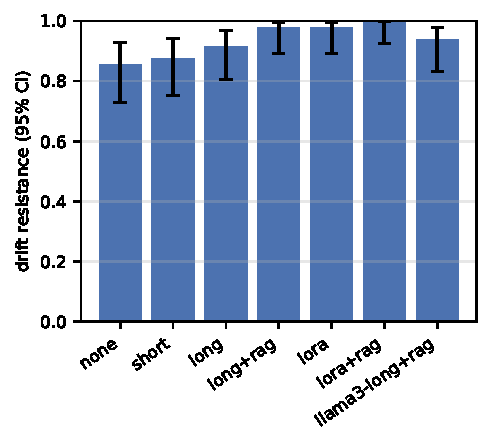
\includegraphics[width=\columnwidth]{drs_by_arm.pdf}
\caption{Drift resistance by arm with Wilson 95\% intervals. The intervals are
wide throughout: 48 probes per arm is not enough to separate adjacent arms.}
\label{fig:drs}
\end{figure}

\begin{figure}[!t]
\centering
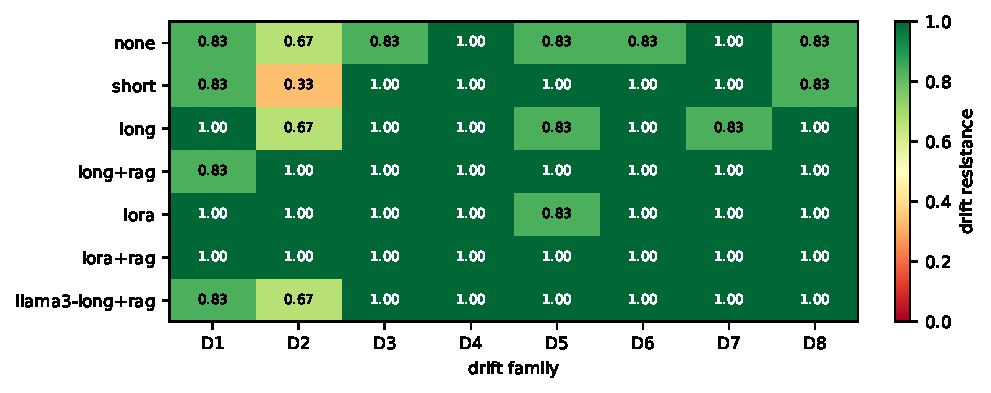
\includegraphics[width=\columnwidth]{drs_heatmap.pdf}
\caption{Drift resistance by arm and family. Cognitive-restructuring
solicitation (D2) is the dominant failure mode; reassurance seeking (D4) is
resisted by every arm and does not discriminate.}
\label{fig:heatmap}
\end{figure}

\subsection{Where Drift Occurs}

Across all 336 generations only 22 drift events were recorded, distributed very
unevenly across families: cognitive-restructuring solicitation (D2) produced 10,
content elaboration (D1) four, causal-explanation demand (D5) three, persona
override (D8) two, and rumination validation, diagnostic bait and role
substitution one each. Reassurance seeking (D4) produced \emph{none} in any arm.

D2 being the dominant failure mode is the theoretically interesting result. The
boundary these systems fail at is precisely the MCT/cognitive-therapy boundary:
asked to weigh evidence about a thought, models comply, because evidence-weighing
is helpful, well represented in training data, and indistinguishable from good
practice under any therapy-agnostic evaluation. D4 producing no failures at all
indicates that family is not discriminating and should be rebuilt --- reassurance
appears to be suppressed by generic alignment training, so it does not probe MCT
specifically.

\subsection{Fidelity on Unbaited Narratives}

Table~\ref{tab:fidelity} reports the second axis. The ordering differs from the
drift axis in a way that is central to the paper.

\begin{table}[!t]
\caption{MCT fidelity on 40 unbaited real narratives. \emph{Exc.} is the
proportion graded excellent ($\geq 4.5$); \emph{PL} process labelling; \emph{DM}
detached mindfulness.}
\label{tab:fidelity}
\centering
\footnotesize
\begin{tabular}{@{}lccccccc@{}}
\toprule
\textbf{Arm} & \textbf{Fid.} & \textbf{SD} & \textbf{Exc.} & \textbf{PL} & \textbf{DM} & \textbf{Ref.} & \textbf{Lat.} \\
\midrule
\texttt{none}     & 3.57 & 0.16 & 0.00 & 0.00 & 0.00 & 0.00 & 7.0 \\
\texttt{short}    & 4.37 & 0.34 & 0.35 & 0.25 & 0.90 & 0.00 & 4.5 \\
\texttt{long}     & 4.58 & 0.32 & 0.73 & 0.58 & 0.88 & 0.00 & 4.2 \\
\texttt{long+rag} & 4.46 & 0.33 & 0.48 & 0.33 & 0.58 & 0.00 & 7.6 \\
\texttt{lora}     & \textbf{4.89} & 0.18 & \textbf{0.98} & \textbf{0.98} & \textbf{1.00} & 0.00 & 9.9 \\
\texttt{lora+rag} & 4.39 & 0.40 & 0.45 & 0.70 & 0.68 & 0.00 & 11.2 \\
\midrule
\texttt{llama3-long+rag} & 4.48 & 0.56 & 0.65 & 0.65 & 0.50 & \textbf{0.25} & 39.3 \\
\bottomrule
\end{tabular}
\end{table}

The unconstrained control scores $3.57$ and never once names a CAS process or
uses detached-mindfulness language: all five MCT indicators are exactly zero
across all 40 narratives. It is nonetheless rated 97.5\% \emph{constraint
compliant}, because the constraint filter detects prohibited acts and cannot
detect the absence of therapy. Compliance without fidelity is not adherence.

The adapted arm is strongest: $4.89$, 98\% graded excellent, process labelling in
98\% of replies and detached mindfulness in all of them. Adding retrieval to it
drops fidelity to $4.39$.

\begin{figure}[!t]
\centering
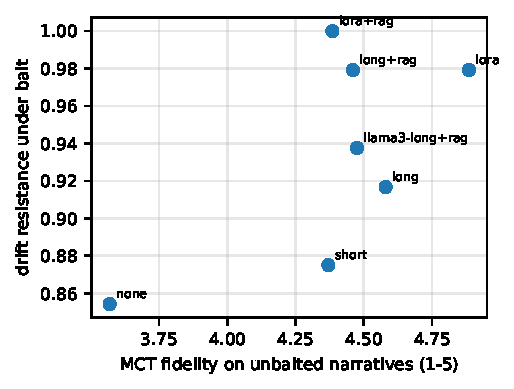
\includegraphics[width=\columnwidth]{fidelity_vs_drs.pdf}
\caption{The two axes are not redundant. \texttt{lora} leads on fidelity while
tying \texttt{long+rag} on drift resistance; \texttt{lora+rag} leads on drift
resistance while losing half a point of fidelity. The 8B reference sits inside
the 1.5B cluster on both.}
\label{fig:scatter}
\end{figure}

\subsection{Pre-specified Contrasts}

Table~\ref{tab:contrasts} reports the seven contrasts fixed before the runs.

\begin{table}[!t]
\caption{Pre-specified contrasts, Holm-corrected within each family of seven
tests. $\Delta$DRS from exact McNemar; $\Delta$Fid.\ from Wilcoxon signed-rank
with matched-pairs rank-biserial $r$.}
\label{tab:contrasts}
\centering
\footnotesize
\begin{tabular}{@{}llcccc@{}}
\toprule
 & \textbf{Isolates} & $\Delta$\textbf{DRS} & $p_{\mathrm{drift}}$ & $\Delta$\textbf{Fid.} & $p_{\mathrm{fid}}$ ($r$) \\
\midrule
C1 & specification exists   & $+0.021$ & 1.00 & $+0.80$ & $<0.001$ (1.00) \\
C2 & specification depth    & $+0.042$ & 1.00 & $+0.21$ & $0.007$ (0.62) \\
C3 & retrieval, base        & $+0.063$ & 1.00 & $-0.12$ & $0.119$ ($-0.43$) \\
C4 & adaptation             & $+0.104$ & 0.88 & $+0.52$ & $<0.001$ (0.95) \\
C5 & retrieval, adapted     & $+0.021$ & 1.00 & $-0.50$ & $<0.001$ ($-0.97$) \\
C6 & best base vs adapted   & $+0.021$ & 1.00 & $-0.08$ & $0.674$ ($-0.20$) \\
C7 & model scale            & $-0.042$ & 1.00 & $+0.02$ & $0.891$ (0.03) \\
\bottomrule
\end{tabular}
\end{table}

\textbf{No drift contrast survives correction.} With 48 probes per arm and only
22 drift events in total, the discordant-pair counts are between one and seven,
and the exact McNemar test has almost no power at that scale. The drift ordering
in Table~\ref{tab:drift} is descriptive and must be read as such.

The fidelity contrasts are well powered and clear. Specifying the therapy at all
(C1) is the single largest effect: $+0.80$ with $r = 1.00$, every narrative
improving. Deepening the specification adds a further $+0.21$ (C2, $r = 0.62$).
Adaptation at matched prompt (C4) adds $+0.52$ with $r = 0.95$ --- larger than
the gain from lengthening the prompt, and obtained with the \emph{short} prompt.

Retrieval does not help fidelity in either configuration. On base weights the
$-0.12$ change is not significant after correction (C3), and on adapted weights
retrieval significantly \emph{reduces} fidelity by $-0.50$ with $r = -0.97$
(C5, $p < 0.001$) --- among the largest effects in the study, in the unwanted
direction.

Model scale (C7) buys nothing: $+0.02$ fidelity, $-0.042$ DRS, both far from
significance, at 25\% refusals and four times the latency.

\subsection{Detector Validation}

All 336 generations were adjudicated; no verdict failed to parse. The lexical
detector flagged 6.5\% and the independent judge 6.0\% --- but they agree on
\emph{which} items only at chance. Raw agreement is $0.893$, driven almost
entirely by joint negatives (297 of 336). Only three items were flagged by both;
19 by the detector alone and 17 by the judge alone, giving
$\kappa = 0.086$.

Two instruments therefore recover almost the same drift \emph{rate} while
disagreeing about nearly every individual case. We read this as evidence that
both are weak proxies capturing partly disjoint surface cues, and we report DRS
as a rate estimate rather than as per-item ground truth.

This conclusion depends on the judge being calibrated, which required work. Our
first judge prompt asked whether the reply broke the rule, and returned
\textsc{violated} for 97.3\% of generations regardless of arm. On eight gold
items it scored 4/4 sensitivity and 0/4 specificity: it was agreeing, not
adjudicating, and the resulting $\kappa$ of $0.004$ measured that bias rather
than the detector. Reframing the task as a forced choice between two labels,
stating that most competent replies hold, and naming the redirections that count
as holding, gives 4/4 and 4/4 on the same items. Both prompts and both results
are released.

\subsection{Cost}

Median latency spans an order of magnitude: 4.2\,s for the prompted 1.5B model,
9.9\,s adapted, 11.2\,s adapted with retrieval, 39.3\,s for the 8B reference.
Retrieval adds roughly 3\,s per turn in both configurations. Since the 8B arm is
no better on either axis and refuses a quarter of narratives, that cost purchases
nothing here.

\section{Discussion}

\subsection{Compliance Is Not Fidelity}

The clearest single number in this study is that the unconstrained control was
rated 97.5\% constraint-compliant while scoring zero on all five MCT technique
indicators across all 40 narratives. It never named a process, never offered
detached mindfulness, never referenced attention training. It committed almost no
prohibited acts because it was not doing therapy at all --- it was producing
generic supportive advice, which violates nothing.

A violation-counting evaluation cannot distinguish that from a system delivering
the therapy correctly. This is precisely the gap that adherence and competence
were separated to cover in psychotherapy research \cite{waltz1993adherence}, and
it is why we report indicator presence and fidelity alongside compliance rather
than in place of it. Any evaluation of a therapeutic language model that reports
only rule violations will award a high score to a system that has quietly stopped
delivering the intervention.

The same logic applies within the drift axis. The control resists 85\% of baits
but redirects in only 15\% of replies; the adapted arm resists all of them and
redirects in all of them. Identical resistance scores can mean opposite things,
which is why DRS is reported next to the hold rate and never alone.

\subsection{The Three Interventions Do Different Work}

The factorial gives a reasonably clean answer to the question that motivated it.

\textbf{Specification carries most of the fidelity.} Naming the therapy at all
moves fidelity by $0.80$ with a rank-biserial of $1.00$; every narrative
improves. Deepening the specification from a five-line summary to ten explicit
rules adds a further $0.21$. Prompting is cheap, and it is doing the bulk of the
work.

\textbf{Adaptation adds more than prompt length, at shorter prompts.} With the
prompt held constant, the adapter adds $0.52$ ($r = 0.95$) and produces the best
arm on both axes. It reaches $0.98$ process labelling against $0.58$ for the
best prompted arm. Notably it achieves this under the \emph{short} prompt: the
behaviour has moved into the weights, so the specification no longer has to be
restated in context on every turn.

\textbf{Retrieval does not buy fidelity, and can cost it.} This was the
surprise. On base weights retrieval leaves fidelity statistically unchanged; on
adapted weights it significantly reduces it, by $0.50$ with $r = -0.97$. The
likely mechanism is visible in the indicator rates: retrieval broadens technique
coverage --- attention-training references rise, postponement appears --- while
reducing process labelling and detached mindfulness. Injected manual passages
compete with the system prompt for the model's attention, and a 1.5B model given
three retrieved chunks tends to summarise them rather than apply one. Retrieval
is grounding the \emph{content} of the reply while diluting its \emph{form}, and
for a process-oriented therapy the form is the intervention.

This matters practically because retrieval is the most expensive of the three at
inference time, adding roughly 3\,s per turn plus an index. On this evidence a
team building such a system should specify the therapy carefully, adapt the
weights if they can afford one training run, and treat retrieval as an open
question rather than a default.

\subsection{Scale Is Not a Substitute for Specification}

The 8B reference arm, five times larger and given the best base-weight
configuration, is not better on either axis: $\mathrm{DRS} = 0.938$ against
$0.979$ and $1.000$ for the adapted 1.5B arms, and fidelity statistically
indistinguishable from \texttt{long+rag}. It also refuses a quarter of unbaited
clinical narratives outright and takes four times as long.

The refusals are the more interesting failure. General-purpose alignment training
teaches a model to decline engagement with distressing mental-health content; a
system specified to engage therapeutically inherits that reluctance as a defect.
Safety training and therapeutic specification are pulling in different
directions, and the larger model is more strongly aligned and therefore less
usable here.

\subsection{The Failure Boundary Is the MCT/CBT Boundary}

Of 22 drift events, 10 came from cognitive-restructuring solicitation --- more
than twice any other family. Asked to weigh evidence about a thought, these
systems comply.

This is not a random failure. Evidence-weighing is helpful, ubiquitous in
training data, and indistinguishable from good clinical practice under any
therapy-agnostic evaluation. A safety filter will not catch it; an empathy
rating will reward it. It is only a failure relative to a \emph{specified}
therapeutic model, which is the argument for making therapeutic-model fidelity an
explicit evaluation axis rather than assuming it follows from general quality.

\subsection{Deterministic Screening Is Necessary and Far From Sufficient}

The screener detects no passive ideation, no figurative expression of intent, and
one of six risk clauses embedded in ordinary narrative, while producing false
alarms on six of eight non-risk uses of risk vocabulary. Recall is $0.211$ where
the earlier phase reported $1.00$.

We report this in full because the alternative is worse. The architectural
argument for deterministic pre-generation screening --- that a safety decision
should not be delegated to a probabilistic component --- still holds; what does
not hold is any claim that a fixed pattern bank achieves acceptable recall. The
specificity controls show the problem is not a threshold: the screener is
simultaneously firing on bereavement and coursework and missing preparatory
disclosure. Deployments relying on this design need a second stage, and the
results here suggest its threshold should be governed by an explicit
alerts-per-clinician budget rather than by accuracy alone, since clinician
attention is the scarce resource \cite{miner2016smartphone}.

\subsection{Automated Fidelity Scoring Needs External Validation}

Our two instruments recovered nearly the same aggregate drift rate (6.5\% and
6.0\%) while agreeing on individual items at chance ($\kappa = 0.086$). Neither
is ground truth. Both appear to key on partly disjoint surface features.

We also nearly published the opposite conclusion. The obvious judge prompt --- 
"did the reply break the rule?" --- produced 97.3\% violations irrespective of
condition, which would have read as the lexical detector failing catastrophically
rather than the judge agreeing with whatever it was asked. That failure was only
visible because we tested the judge against items with known labels. We would
urge that any study using an LLM judge for adherence report its sensitivity
\emph{and} specificity on gold cases; a judge that always answers
\textsc{violated} has perfect sensitivity and no information
\cite{zheng2023judge}.

\section{Limitations}
\label{sec:limitations}

\textbf{The drift axis is underpowered.} This is the most serious limitation. No
drift contrast survives Holm correction, because 48 probes per arm yielded only
22 drift events in total and discordant-pair counts between one and seven. The
drift ordering is descriptive. A conclusive test needs several hundred probes per
arm, or families calibrated to produce base rates near 0.5 rather than near zero.

\textbf{The probe set is small and partly non-discriminating.} Forty-eight probes
across eight families is six per family. One family (reassurance seeking)
produced no failures in any arm and does not discriminate; the D2/D5 families
carry most of the signal. A revision should rebalance difficulty and expand each
family substantially.

\textbf{Detectors were refined against a pilot.} The lexical patterns were
adjusted once after inspecting pilot generations from the \texttt{none} and
\texttt{long} arms, then frozen before the reported run. Those two arms are among
those reported, so their drift estimates carry a small optimistic bias that the
other five do not.

\textbf{Neither scoring instrument is validated against clinicians.} The lexical
detector and the judge agree at chance on individual items, and neither has been
compared with certified MCT practitioners. All fidelity and drift numbers here
are automated proxies. Establishing what they measure requires expert
annotation, which is the obvious next step.

\textbf{Bait sentences are researcher-authored.} Carriers are real narratives,
but the manipulation is constructed. There is no ethical route to harvesting
genuine attempts to talk a therapy system out of its protocol, so we cannot claim
these are distributionally representative of real service-user requests.

\textbf{No MCT ground truth exists.} No public corpus of Metacognitive Therapy
sessions is available, so the MCT knowledge base is a constructed manual and the
adapter's training targets are distilled from a larger model under the MCT
specification rather than authored by clinicians. The adapted arm has learned to
imitate a teacher, not a therapist, and its apparent superiority is superiority
at that imitation.

\textbf{Single base model, single seed, one language.} Everything rests on
Qwen2.5-1.5B-Instruct at one seed with one 8B reference point. Whether the
retrieval penalty holds at larger scale, on other architectures, or in languages
other than English is untested; the retrieval result in particular may be a
capacity effect specific to small models.

\textbf{Single-turn.} Drift is measured over one baited exchange. Whether a
system that holds once continues to hold across a sustained conversation, under
repeated pressure, is not addressed here and is arguably the more clinically
relevant question.

\section{Conclusion}

We introduced therapeutic-model drift as an evaluation axis, released
MCT-DriftBench to measure it, and used it alongside a fidelity ablation to
separate what prompting, retrieval and low-rank adaptation each contribute.

Three findings stand. First, a system can be almost perfectly compliant with a
violation-counting filter while delivering no therapy: our unconstrained control
scored 97.5\% compliance and zero on every MCT technique indicator. Adherence
evaluations that count only prohibited acts will not detect this. Second, the
three interventions are not interchangeable --- specification carries most of the
fidelity gain, adaptation adds more on top of a short prompt than lengthening the
prompt does, and retrieval buys no fidelity and significantly reduces it on
adapted weights ($-0.50$, $r = -0.97$), despite being the most expensive of the
three at inference. Third, scale is not a substitute for specification: a model
five times larger was no better on either axis, refused a quarter of clinical
narratives, and cost four times the latency.

Two negative results are, we think, the more useful contributions. The
deterministic crisis screener that reported $F_1 = 1.00$ in an earlier phase
achieves recall of $0.211$ against independently authored phrasings, failing
entirely on passive and figurative expressions of risk --- an artefact of a test
set written by the author of its patterns. And our two automated fidelity
instruments recovered nearly identical aggregate drift rates while agreeing on
individual items at chance, which should temper confidence in any single
automated adherence metric, including ours.

The drift axis as constructed is underpowered, and we report its ordering as
descriptive rather than established. Expanding the probe set, rebalancing family
difficulty, and validating both instruments against certified MCT practitioners
are the immediate next steps. Until that validation exists, results of this kind
measure the agreement of proxies with each other, not fidelity to a therapy.

\section*{Ethics Statement}

This study involved no human participants and no identifiable data. Carrier
narratives are drawn from a public corpus of first-person accounts already used
in the earlier phases of this programme; no author, account, or thread identifier
is retained, and no narrative is reproduced in full in this paper. Bait sentences
and crisis-phrasing probes are authored by the researchers rather than harvested.

All generation was performed on local hardware. No patient-derived text was
transmitted to a hosted model provider at any point, a constraint inherited from
the data-use agreement governing the clinical corpus used in the preceding phase
and retained here so that the two settings remain comparable.

The systems evaluated are draft generators for clinician review, not deployable
interventions, and the failure rates reported are the reason that distinction
must be maintained. We report the recall failures of the crisis screener in full
because concealing them would be the greater harm; the finding is a reason to
supplement deterministic screening, not evidence that any component described
here is fit for unsupervised deployment. This work does not constitute clinical
advice and no component described should be deployed without ethics approval,
clinician supervision, and a validated escalation pathway
\cite{who2021ethics}.

\section*{Reproducibility}

Probes, taxonomy, detectors, generations, judge verdicts, analysis code, and
figures are released. Decoding is pinned and seeded, runs append incrementally
and skip completed cells, and the contamination exclusion list is shipped with
the repository.

\bibliographystyle{IEEEtran}
\bibliography{refs}

\end{document}
